% Created 2024-06-24 Mon 02:03
% Intended LaTeX compiler: pdflatex
\documentclass[11pt]{article}
\usepackage[utf8]{inputenc}
\usepackage[T1]{fontenc}
\usepackage{graphicx}
\usepackage{longtable}
\usepackage{wrapfig}
\usepackage{rotating}
\usepackage[normalem]{ulem}
\usepackage{amsmath}
\usepackage{amssymb}
\usepackage{capt-of}
\usepackage{hyperref}
\usepackage[a4paper,left=1cm,right=1cm,top=1cm,bottom=1cm]{geometry}
\usepackage[american, english]{babel}
\usepackage{enumitem}
\usepackage{float}
\usepackage[sc]{mathpazo}
\linespread{1.05}
\renewcommand{\labelitemi}{$\rhd$}
\setlength\parindent{0pt}
\setlist[itemize]{leftmargin=*}
\setlist{nosep}
\author{Marcio Woitek}
\date{}
\title{Approximations for Metric TSPs}
\hypersetup{
 pdfauthor={Marcio Woitek},
 pdftitle={Approximations for Metric TSPs},
 pdfkeywords={},
 pdfsubject={},
 pdfcreator={Emacs 29.3 (Org mode 9.8)}, 
 pdflang={English}}
\begin{document}

\maketitle
\thispagestyle{empty}
\pagestyle{empty}

Problems 1-4 are related to the figure below.
\begin{figure}[H]
  \centering
  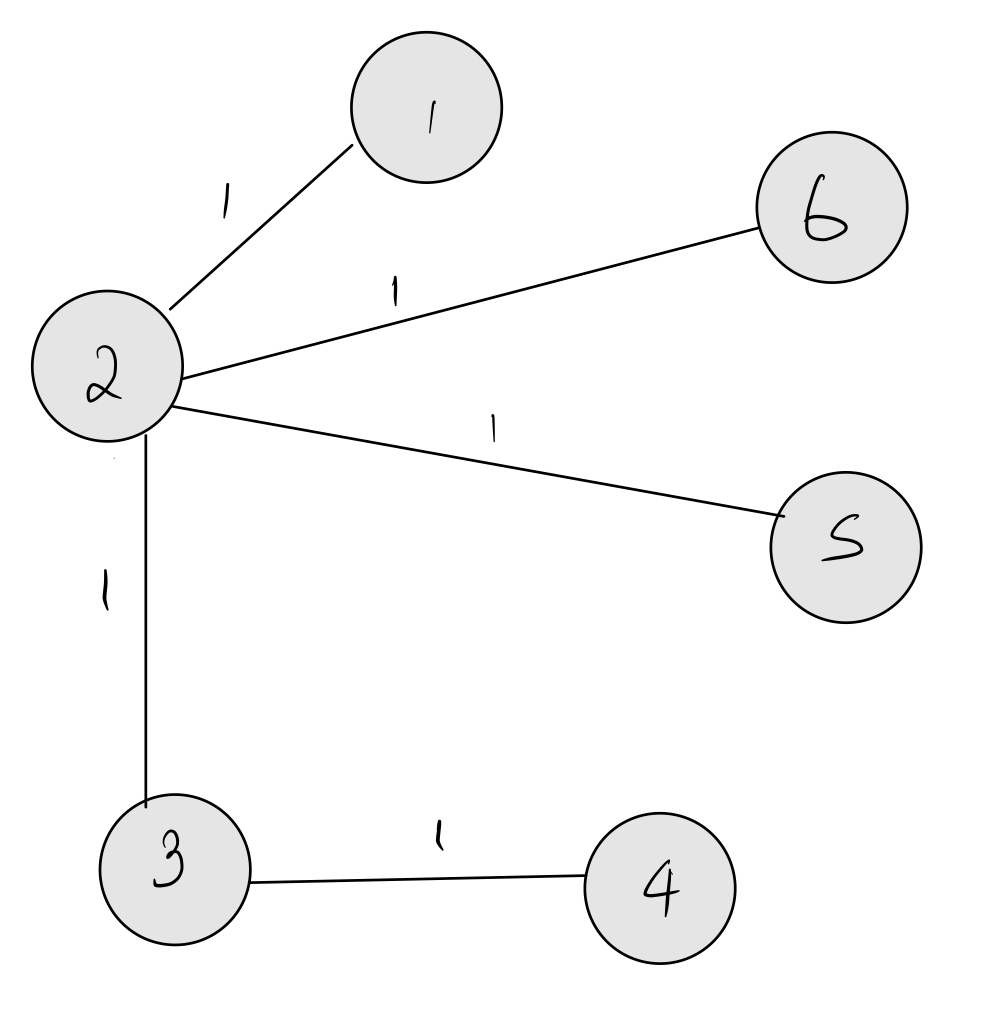
\includegraphics[scale=0.15]{tsp_mst_quiz.jpeg}
  \caption{Minimum spanning tree for some TSP instance}
\end{figure}
\section*{Problem 1}
\label{sec:org46250a8}
\begin{itemize}
\item \((4,1)\)
\item \((5,6)\)
\item \((6,3)\)
\end{itemize}
\section*{Problem 2}
\label{sec:org376a94a}
\begin{itemize}
\item \(C_{6,5}=C_{5,6}\)
\item \(C_{6,5}\leq 2\)
\end{itemize}
\section*{Problem 3}
\label{sec:org344f08b}
\begin{itemize}
\item The cost of the tour must be less than or equal to twice the cost of the MST.
\item The cost of the TSP tour must be \(\leq 10\).
\end{itemize}
\section*{Problem 4}
\label{sec:org1e973fc}
\begin{itemize}
\item The optimal tour cost has to be \(\geq 5\).
\item The optimal tour cost has to be \(\leq 10\).
\end{itemize}

\newpage

The next two problems are related to this graph:
\begin{figure}[H]
  \centering
  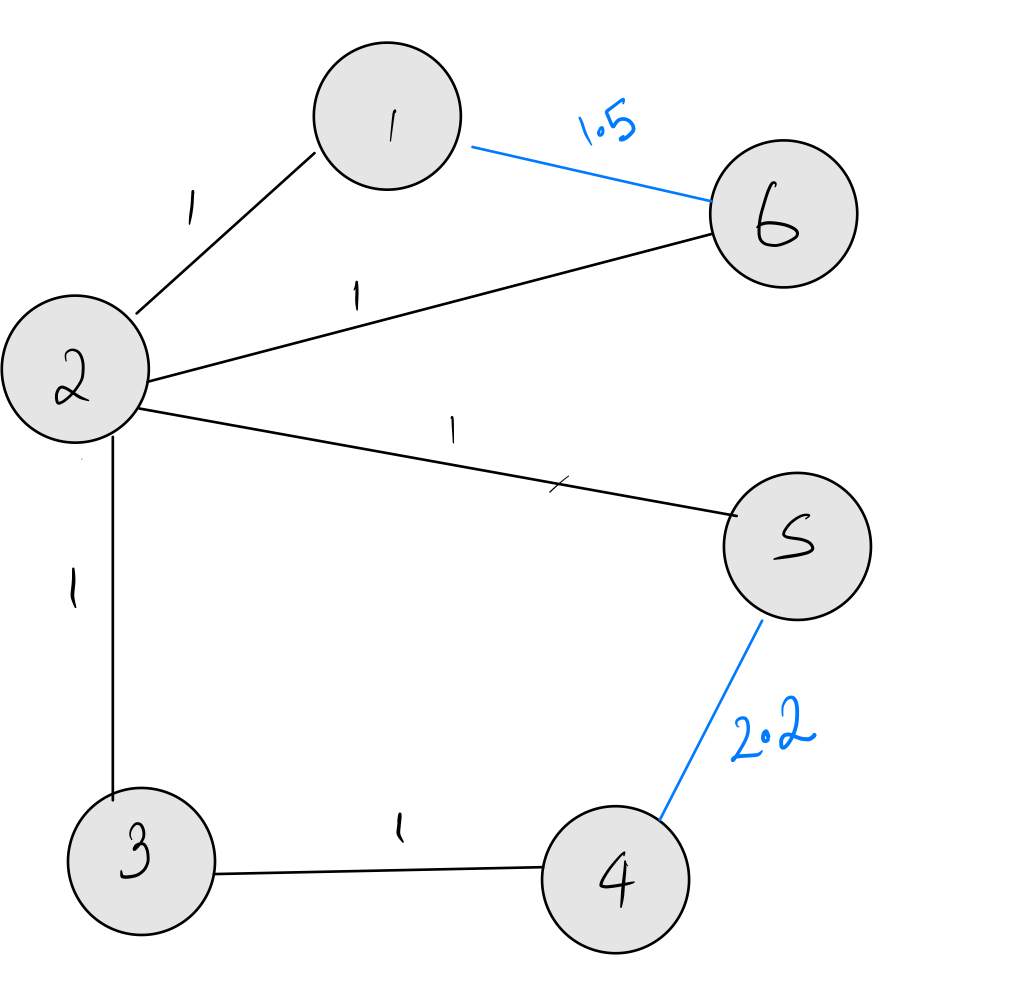
\includegraphics[scale=0.15]{tsp_mst_with_matching.jpeg}
  \caption{Graph for Problems 5 and 6}
\end{figure}
\section*{Problem 5}
\label{sec:orgdafc2e8}
\textbf{Answer: \([1,2,5,4,3,6]\)}
\section*{Problem 6}
\label{sec:orga9ea1a4}
\begin{itemize}
\item Cost of TSP tour is less than or equal to 8.7.
\item The cost of the tour must be less than or equal to the cost of all the edges
in the matching + cost of all edges in the MST.
\item Cost of TSP tour is less than or equal to 10 (the bound we placed on the cost
of the previous tour using DFS).
\end{itemize}
\end{document}
